\حصہ{ایک سے زائد بلا منصوبہ متغیرات کی تقسیمیں}
اگر ایک بلا منصوبہ تجربہ میں ہم ایک مقدار کا مشاہدہ کریں تب ہمیں اس تجربہ کے ساتھ واحد ایک بلا منصوبہ متغیر، مثلاً \عددی{X}، وابستہ کرنا ہو گا۔حصہ \حوالہ{حصہ_شماریات_بلا_منصوبہ_متغیرات} سے ہم جانتے ہیں کہ اس کا مطابقتی تفاعل تقسیم \عددی{F(x)=P(X\le x)} اس تقسیم کو مکمل طور پر تعین کرتا ہے، چونکہ ہر وقفہ \عددی{a<X\le b} کے لئے درج ذیل ہو گا۔
\begin{align*}
P(a<X\le b)=F(b)-F(a)
\end{align*}

اگر ایک بلا منصوبہ تجربہ میں ہم دو مقدار کا مشاہدہ کریں تب ہمیں اس تجربہ کے ساتھ دو بلا منصوبہ متغیرات، مثلاً \عددی{X} اور \عددی{Y}، وابستہ کرنا ہو گا۔مثال کے طور پر فولاد کی راک ویل سختی کو  \عددی{X}  اور اس میں کاربن کی مقدار کو \عددی{Y} ظاہر کر سکتے ہیں۔ہر ایک تجربہ اعداد کی جوڑی \عددی{X=x}، \عددی{Y=y} دے گی جس کو مختصراً \عددی{(x,y)} لکھا اور \عددی{XY} مستوی پر بطور نقطہ دکھایا جا سکتا ہے۔ہم اب ایک مستطیل \عددی{a_1<X\le b_1}، \عددی{a_2<Y\le b_2} پر غور کرتے ہیں (شکل \حوالہ{شکل_شماریات_دو_بعدی_تقسیم})۔اگر ایسے ہر ایک مستطیل کے لئے  ہمیں مطابقتی احتمال
\begin{align*}
P(a_1<X\le b_1,\,\, a_2<Y\le b_2)
\end{align*}
معلوم ہو تب ہم کہتے ہیں کہ \اصطلاح{دو بعدی بلا منصوبہ متغیر}\فرہنگ{بلا منصوبہ!دو بعدی متغیر}\حاشیہب{two-dimensional random variable}\فرہنگ{random!two-dimensional variable} \عددی{(X,Y)} یا بلا منصوبہ متغیرات \عددی{X} اور \عددی{Y} کا \اصطلاح{دو بعدی تفاعل احتمال}\فرہنگ{احتمال!دو بعدی تفاعل}\حاشیہب{two-dimensional probability distribution}\فرہنگ{probability!two-dimensional function} ہمیں معلوم ہے۔تفاعل
\begin{align}\label{مساوات_شماریات_ایک_سے_زائد_الف}
F(x,y)=P(X\le x,Y\le y)
\end{align}
کو اس تقسیم یا \عددی{(X,Y)} کا \اصطلاح{تقسیمی تفاعل}\فرہنگ{تقسیمی!تفاعل}\حاشیہب{distribution function}\فرہنگ{distribution!function} کہتے ہیں۔چونکہ (سوال \حوالہ{سوال_شماریات_ایک_سے_زائد_ثبوت_ب})
\begin{gather}
\begin{aligned}\label{مساوات_شماریات_ایک_سے_زائد_ب}
P(a_1&<X\le b_1,a_2<Y\le b_2)\\
&=F(b_1,b_2)-F(a_1,b_2)-F(b_1,a_2)+F(a_1,a_2)
\end{aligned}
\end{gather}
لکھا جا سکتا ہے لہٰذا مساوات \حوالہ{مساوات_شماریات_ایک_سے_زائد_الف} تقسیم کو یکتا طور پر تعین کرتا ہے۔
\begin{figure}
\centering
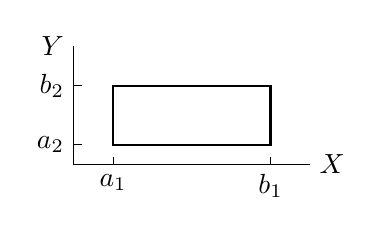
\begin{tikzpicture}
\draw(0,1.5)node[left]{$Y$}--(0,0)--(3,0)node[right]{$X$};
\draw[thick](0.5,0.25) rectangle (2.5,1);
\draw(0.5,0)node[below]{$a_1$}--++(0,0.1);
\draw(2.5,0)node[below]{$b_1$}--++(0,0.1);
\draw(0,0.25)node[left]{$a_2$}--++(0.1,0);
\draw(0,1)node[left]{$b_2$}--++(0.1,0);
\end{tikzpicture}
\caption{دو بعدی تقسیم کا تصور}
\label{شکل_شماریات_دو_بعدی_تقسیم}
\end{figure}

%==================
\جزوحصہء{غیر مسلسل دو بعدی تقسیمیں}
اگر \عددی{(X,Y)} درج ذیل خواص رکھتا ہو تب متغیر \عددی{(X,Y)} اور اس کا مطابقتی تقسیم \اصطلاح{غیر مسلسل}\فرہنگ{غیر مسلسل!تقسیم}\فرہنگ{غیر مسلسل!متغیر}\فرہنگ{discrete!variable}\فرہنگ{discrete!distribution} کہلائے گا۔

\عددی{X,Y} متناہی تعداد یا قابل شمار لامتناہی تعداد کی جوڑی قیمتیں \عددی{(x,y)} اختیار کر سکتا ہے جن کے مطابقتی احتمال مثبت ہوں گے۔ہر ایسا دائرہ کار جس میں ایسی کوئی جوڑی نہ پائی جاتی ہو کا احتمال \عددی{0} ہو گا\حاشیہد{دھیان رہے کہ پہلی خاصیت سے یہ نہیں کہا جا سکتا ہے}۔ 

فرض کریں کہ \عددی{x_i,y_j} ایسی کوئی  جوڑی ہے اور \عددی{P(X=x_i,Y=y_j)=p_{ij}} ہے(جہاں ہم فرض کرتے ہیں کہ \عددی{p_{ij}} کسی مخصوص \عددی{i,j} کی جوڑیوں  کے لئے صفر بھی ہو سکتا ہے)۔ تفاعل
\begin{align}
f(x,y)=
\begin{cases}
p_{ij}& x=x_i,y=y_j\\
0&\text{ورنہ}
\end{cases}
\end{align}
کو \عددی{(X,Y)} کا \اصطلاح{تفاعل احتمال} کہتے ہیں؛ یہاں غیر تابع طور پر \عددی{i=1,2,\cdots} اور \عددی{j=1,2,\cdots} ہیں۔مساوات \حوالہ{مساوات_شماریات_غیر_مسلسل_متغیر_ج} کا مماثل 
\begin{align}
F(x,y)=\sum_{x_i\le x}\sum_{y_j\le y}f(x_i,y_j)
\end{align}
ہے اور مساوات \حوالہ{مساوات_شماریات_غیر_مسلسل_متغیر_پ} کی جگہ درج ذیل شرط ہو گا۔
\begin{align}
\sum_{i}\sum_{j}f(x_i,y_j)=1
\end{align}

مثال کے طور پر اگر ہم ایک روپیہ اور پانچ روپیہ کے سکے اچھال کر 
\begin{align*}
X&=\text{\RL{ایک روپیہ کی خط کی تعداد}}\\
Y&=\text{\RL{پانچ روپیہ کی خط کی تعداد}}
\end{align*}
پر غور کریں تب \عددی{X} اور \عددی{Y} کی قیمت\عددی{0} یا \عددی{1} ہو سکتی ہے اور تفاعل احتمال
\begin{align*}
\text{\RL{ہو گا۔}}\,\, f(x,y)=0\,\,\text{\RL{ورنہ (ان کے علاوہ)}}\,\,f(0,0)=f(1,0)=f(0,1)=f(1,1)=\frac{1}{4}
\end{align*}

%======================
\جزوحصہء{استمراری دو بعدی تقسیمیں}
\عددی{(X,Y)} اور اس کا تقسیم اس صورت استمراری کہلاتے ہیں جب  مطابقتی تفاعل تقسیم کو دوہرا تکمل
\begin{align}
F(x,y)=\int_{-\infty}^{y}\int_{-\infty}^{x}f(x^*,y^*)\dif x^*\dif y^*
\end{align}
کی صورت میں لکھنا ممکن ہو جہاں \عددی{f(x,y)} معین، غیر منفی اور پورے مستوی میں محدود ہے ماسوائے متناہی تعداد کے استمراری قابل تفرق منحنیات پر۔ \عددی{f(x,y)} کو تقسیم کی \اصطلاح{کثافت احتمال} کہتے ہیں۔یوں درج ذیل ہو گا۔
\begin{align}
P(a_1<X\le b_1, a_2<Y\le b_2)=\int_{a_2}^{b_2}\int_{a_1}^{b_1}f(x,y)\dif x\dif y
\end{align}

مثال کے طور پر  (شکل \حوالہ{شکل_شماریات_یکساں_تقسیم_الف})
\begin{align}\label{مساوات_شماریات_یکساں_متعدد_متغیرات_کثافت}
f(x,y)=0\,\text{ورنہ}\,f(x,y)=\frac{1}{k}\,\text{میں ہو تب}\,R\,\text{\RL{مستطیل}} \,(x,y)\,\text{جب}
\end{align}
مستطیل \عددی{R} میں یکساں تقسیم کو ظاہر کرتا ہے؛ یہاں \عددی{k} مستطیل کا رقبہ یعنی \عددی{k=(\beta_1-\alpha_1)(\beta_2-\alpha_2)} ہے۔اس تقسیم کو شکل \حوالہ{شکل_شماریات_یکساں_تقسیم_ب} میں دکھایا گیا ہے۔
\begin{figure}
\centering
\begin{minipage}{0.45\textwidth}
\centering
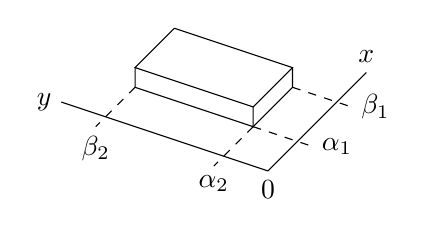
\begin{tikzpicture}[x={(-0.5cm,-0.5cm)},y={(0.75cm,-0.25cm)},z={(0,1cm)}]
\draw(0,0,0.25)--++(1,0,0)--++(0,2,0)--++(-1,0,0)--++(0,-2,0);
\draw(1,0,0.25)--++(0,0,-0.25)--++(0,2,0)--++(0,0,0.25);
\draw(1,2,0)--++(-1,0,0)--++(0,0,0.25);
\draw[dashed] (1,0,0)--++(1,0,0)node[below]{$\beta_2$};
\draw[dashed] (1,2,0)--++(1,0,0)node[below]{$\alpha_2$};
\draw[dashed](0,2,0)--++(0,1,0)node[right]{$\beta_1$};
\draw[dashed](1,2,0)--++(0,1,0)node[right]{$\alpha_1$};
\draw (1.75,2.75)node[below]{$0$}--++(-2.5,0,0)node[above]{$x$};
\draw (1.75,2.75)--++(0,-3.5,0)node[left]{$y$};
\end{tikzpicture}
\caption{یکساں تقسیم (مساوات \حوالہ{مساوات_شماریات_یکساں_متعدد_متغیرات_کثافت}) کا تفاعل احتمال کثافت}
\label{شکل_شماریات_یکساں_تقسیم_الف}
\end{minipage}\hfill
\begin{minipage}{0.45\textwidth}
\centering
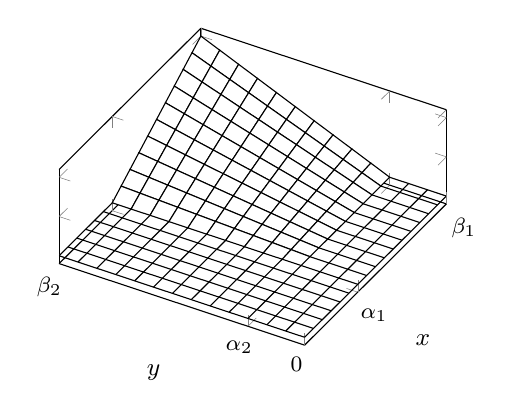
\begin{tikzpicture}
\begin{axis}[small, view={-60}{60},xtick={0.6,1.6},ytick={0,0.6,2.6},xticklabels={$\alpha_1$,$\beta_1$},yticklabels={$0$,$\alpha_2$,$\beta_2$},zticklabels={\empty},xlabel={$x$},ylabel={$y$}]
\addplot3[samples=11,samples y=11,surf,color=white,faceted color=black,domain=0.6:1.6,y domain=0.6:2.6]{(x-0.6)*(y-0.6)};
%the following manually matches the grid lines
\foreach \kk in {0.6,0.8,...,2.6}{
\addplot3 [domain=0:0.6, samples y=1, black,smooth] (x,\kk,0);}
\foreach \kk in {0.6,0.7,...,1.6}{
\addplot3 [domain=0:0.6, samples y=1, black,smooth] (\kk,x,0);}
\foreach \kk in {0,0.2,...,0.58}{
\addplot3 [domain=0:1.6, samples y=1, black,smooth] (x,\kk,0);}
\foreach \kk in {0,0.1,...,0.59}{
\addplot3 [domain=0:2.6, samples y=1, black,smooth] (\kk,x,0);}
\end{axis}
\end{tikzpicture}
\caption{یکساں تقسیم (مساوات \حوالہ{مساوات_شماریات_یکساں_متعدد_متغیرات_کثافت}) کا تفاعل تقسیم}
\label{شکل_شماریات_یکساں_تقسیم_ب}
\end{minipage}%
\end{figure}

%=================
\جزوحصہء{دو بعدی غیر مسلسل تقسیم کے حاشیہ تقسیمیں}
فرض کریں کہ بلا منصوبہ غیر مسلسل متغیر \عددی{(X,Y)} کا تفاعل احتمال \عددی{f(x,y)} ہے۔اگر \عددی{X=x} ہو، جبکہ \عددی{Y} جس میں ہمیں دلچسپی نہیں ہے کوئی بھی قیمت اختیار کر سکتا ہو، تب تفاعل احتمال \عددی{P(X=x,Y \text{اختیاری})} کو \عددی{f_1(x)} لکھا جا سکتا ہے جو \عددی{x} کا تابع تفاعل ہے۔یوں 
\begin{align}\label{مساوات_شماریات_حاشیہ_الف}
f_1(x)=P(X=x,Y\,\text{اختیاری})=\sum_y f(x,y)
\end{align} 
لکھا جا سکتا ہے جہاں اس \عددی{x} کے لئے ہم \عددی{f(x,y)} کی  تمام غیر صفر قیمتوں کا مجموعہ لیا گیا ہے۔ظاہر ہے کہ \عددی{f_1(x)} ایک بلا منصوبہ متغیر تقسیمی احتمال کا تفاعل احتمال ہے۔اس تقسیم کو دیے گئے دو بعدی تقسیم کے لحاظ ہے \عددی{X} کا \اصطلاح{حاشیہ تقسیم}\فرہنگ{تقسیم!حاشیہ}\حاشیہب{marginal distribution}\فرہنگ{distribution!marginal} کہا جاتا ہے۔اس کا تفاعل تقسیم درج ذیل ہو گا۔
\begin{align}\label{مساوات_شماریات_حاشیہ_ب}
F_1(x)=P(X\le x,Y\, \text{اختیاری})=\sum_{x^*\le x} f_1(x^*)
\end{align}
اسی طرح تفاعل احتمال 
\begin{align}\label{مساوات_شماریات_حاشیہ_پ}
f_2(y)=P(X\,\text{اختیاری}, Y=y)=\sum_x f(x,y))
\end{align}
دیے گیے دو بعدی تقسیم کا \عددی{Y} کے لحاظ سے \اصطلاح{حاشیہ تقسیم} تعین کرتا ہے۔مساوات \حوالہ{مساوات_شماریات_حاشیہ_پ} میں ہم \عددی{y} کے مطابقتی غیر صفر \عددی{f(x,y)} کا مجموعہ لیتے ہیں۔اس تقسیم کا تفاعل تقسیم درج ذیل ہو گا۔
\begin{align}
F_2(y)=P(X\,\text{اختیاری},Y\le y)=\sum_{y^*\le y}f_2(y^*)
\end{align}
ظاہر ہے کہ بلا منصوبہ متغیر \عددی{(X,Y)} کے دونوں حاشیہ تقسیم  غیر مسلسل ہیں۔

جدول \حوالہ{جدول_شماریات_تاش_ملکہ_بادشاہ} میں ان کی مثال دی گئی ہے جہاں تاش کے پتوں سے تین پتے نکال کر واپس رکھے جاتے ہیں۔ملکہ کے حصول کو \عددی{X} جبکہ بادشاہ کے حصول کو \عددی{Y} سے ظاہر کیا گیا ہے۔تاش کے کل \عددی{52} پتے ہوتے ہیں جن میں \عددی{4} ملکہ اور \عددی{4} بادشاہ کے پتے ہوتے ہیں۔یوں ایک پتہ نکال کر ملکہ حاصل کرنے کا احتمال \عددی{\tfrac{4}{52}=\tfrac{1}{13}} ہو گا۔یوں ایک پتہ نکال کر ملکہ یا بادشاہ حاصل کرنے کا احتمال \عددی{\tfrac{2}{13}} ہو گا۔اس طرح اس بلا منصوبہ تجربہ کا مطابقتی تفاعل احتمال
\begin{align*}
f(x,y)=\frac{3!}{x!y!(3-x-y)!}\big(\frac{1}{13}\big)^x\big(\frac{2}{13}\big)^y\big(\frac{10}{13}\big)^{3-x-y}\quad \quad (x+y\le 3)
\end{align*}
ہو گا اور ان کے علاوہ \عددی{f(x,y)=0} ہو گا۔جدول \حوالہ{جدول_شماریات_تاش_ملکہ_بادشاہ} میں \عددی{f(x,y)}، \عددی{f_1(x)} اور \عددی{f_2(y)} دیے گئے ہیں۔ 
\begin{table}
\caption{تاش سے ملکہ اور بادشاہ کا حصول}
\label{جدول_شماریات_تاش_ملکہ_بادشاہ}
\centering
\begin{otherlanguage}{english}
\begin{tabular}{C|CCCC||C}
\phantom{xxx}y&\multirow{2}{*}{0}&\multirow{2}{*}{1}&\multirow{2}{*}{2}&\multirow{2}{*}{3}&\multirow{2}{*}{$f_1(x)$}\\
x\phantom{xxx}&&&&&\\
\hline\Tstrut
0&\frac{1000}{2197}&\frac{600}{2197}&\frac{120}{2197}&\frac{8}{2197}&\frac{1728}{2197}\\  \Tstrut \Bstrut \Tstrut \Bstrut
1&\frac{300}{2197}&\frac{120}{2197}&\frac{12}{2197}&0&\frac{432}{2197}\\   \Tstrut \Bstrut   \Tstrut \Bstrut
2&\frac{30}{2197}&\frac{6}{2197}&0&0&\frac{36}{2197}\\   \Tstrut \Bstrut   \Tstrut \Bstrut
3&\frac{1}{2197}&0&0&0&\frac{1}{2197}\\ 
\hline
\hline   \Tstrut \Bstrut
f_2(y)&\frac{1331}{2197}&\frac{726}{2197}&\frac{132}{2197}&\frac{8}{2197}&\\  
\hline
\end{tabular}
\end{otherlanguage}
\end{table}

\جزوحصہء{دو بعدی استمراری تقسیم کے حاشیہ تقسیمیں}
اسی طرح کثافت \عددی{f(x,y)} والے  استمراری متغیر \عددی{X,Y} کے لئے ہم 
\begin{align*}
(X\le x, Y\,\text{اختیاری})\quad \text{یا}\quad (X\le x, -\infty <Y<\infty)
\end{align*}
پر غور کر سکتے ہیں جس کا مطابقتی احتمال
\begin{align*}
F_1(x)=P(X\le x, -\infty<Y<\infty)=\int_{-\infty}^{\infty} \big(\int_{-\infty}^{\infty} f(x^*,y)\dif y\big)\dif x^*
\end{align*}
ہو گا جس میں
\begin{align}
f_1(x)=\int_{-\infty}^{\infty} f(x,y)\dif y
\end{align}
لکھتے ہوئے
\begin{align}
F_1(x)=\int_{-\infty}^{\infty} f_1(x^*)\dif x^*
\end{align}
لکھا جا سکتا ہے۔\عددی{f_1(x)}  اور \عددی{F_1(x)} کو بالترتیب دیے گئے استمراری تقسیم کے لحاظ سے حاشیہ تقسیم \عددی{X} کی  \ترچھا{کثافت} اور \ترچھا{تقسیمی تفاعل} کہتے ہیں۔دیے گئے دو بعدی استمراری تقسیم کے لحاظ سے تفاعل
\begin{align}
f_2(y)=\int_{-\infty}^{\infty} f(x,y)\dif x
\end{align}
کو حاشیہ تقسیم \عددی{Y} کی کثافت اور
\begin{align}
F_2(y)=\int_{-\infty}^{\infty} f_2(y^*)\dif y^*=\int_{-\infty}^{\infty}\int_{-\infty}^{\infty} f(x,y^*)\dif x\dif y^*
\end{align}
کو حاشیہ تقسیم \عددی{Y} کا تقسیمی تفاعل کہتے ہیں۔ہم دیکھتے ہیں کہ استمراری تقسیم کے دونوں حاشیہ تقسیم استمراری ہیں۔

\جزوحصہء{بلا منصوبہ متغیرات کی تابعیت اور غیر تابعیت}
دو بعدی \عددی{(X,Y)} تقسیم جس کا تفاعل تقسیم \عددی{F(x,y)} ہو کے بلا منصوبہ متغیرات \عددی{X} اور \عددی{Y} اس صورت \اصطلاح{غیر تابع}\فرہنگ{تابع!غیر}\فرہنگ{independent} کہلاتے ہیں جب تمام \عددی{(x,y)} کے لئے
\begin{align}
F(x,y)=F_1(x)F_2(y)
\end{align}
ہو ورنہ انہیں \اصطلاح{تابع}\فرہنگ{تابع}\فرہنگ{dependent} کہتے ہیں۔


فرض کریں کہ \عددی{X} اور \عددی{Y} دونوں غیر مسلسل  یا دونوں استمراری ہوں۔تب \عددی{X} اور \عددی{Y} اس صورت غیر تابع ہوں گے جب ان کے مطابقتی تفاعل احتمال یا کثافتیں \عددی{f_1(x)} اور \عددی{f_2(y)} درج ذیل کو مطمئن کرتے ہوں۔
\begin{align}
f(x,y)=f_1(x)f_2(y)
\end{align}
مثال کے طور پر جدول \حوالہ{جدول_شماریات_تاش_ملکہ_بادشاہ} میں متغیرات تابع ہیں۔ایک روپیہ اور پانچ روپیہ کے سکے ایک بار  اچھال کر متغیرات
\begin{align*}
X=\text{\RL{ایک روپیہ کے سکے کے خط کی تعداد}},\quad Y=\text{\RL{پانچ روپیہ کے سکے کے خط کی تعداد}}
\end{align*}
\عددی{0} یا \عددی{1} قیمت اختیار کر سکتے ہیں اور یہ متغیرات غیر تابع ہیں۔

تابعیت اور غیر تابعیت کی تصور کو \عددی{n} بعدی تقسیم \عددی{X_1,\cdots,X_n} جس کا تفاعل احتمال
\begin{align*}
F(x_1,\cdots,x_n)=P(X_!\le x_1,\cdots X_n\le x_n)
\end{align*}
ہو کے \عددی{n} بلا منصوبہ متغیرات  تک وسعت دی جا سکتی ہے۔اگر تمام \عددی{x_1,\cdots,x_n} کے لئے
\begin{align}
F(x_1,\cdots,x_n)=F_1(x_1)F_2(x_2)\cdots F_n(n)
\end{align}
ہو جہاں \عددی{X_j} کے حاشیہ تقسیم کا تقسیمی تفاعل \عددی{F_j(x_j)} ہو، یعنی
\begin{align*}
F_j(x_j)=P(X_j\le x_j, X_k\, \text{اختیاری},\, k\ne j)
\end{align*}
تب یہ بلا منصوبہ متغیرات \اصطلاح{غیر تابع} کہلاتے ہیں ورنہ  ان متغیرات کو \اصطلاح{تابع} کہتے ہیں۔

\جزوحصہء{بلا منصوبہ متغیرات کے تفاعل}
فرض کریں کہ بلا منصوبہ متغیر \عددی{(X,Y)} کا تفاعل احتمال یا کثافت \عددی{f(x,y)} اور تقسیمی تفاعل \عددی{F(x,y)} ہیں اور فرض کریں کہ \عددی{g(x,y)} غیر مستقل استمراری تفاعل ہے جو تمام \عددی{(x,y)} پر معین ہے۔تب \عددی{Z=g(X,Y)} بھی بلا منصوبہ متغیر ہو گا۔مثال کے طور پر ہم دو پانسہ پھینکتے ہیں۔پہلے پانسہ عدد \عددی{X} اور دوسرا پانسہ عدد \عددی{Y} دیتا ہے۔ عدد \عددی{Z=X+Y} ان دونوں کا مجموعہ ہے (شکل \حوالہ{شکل_شماریات_تفاعل_تقسیم_ب})۔

اگر \عددی{(X_1,\cdots,X_n) بلا منصوبہ \عددی{n}} بعدی متغیر ہوا ور تمام \عددی{(x_1,\cdots,x_n)} پر  \عددی{g(x_1,\cdots,x_n)} معین غیر مستقل استمراری تفاعل ہو  تب \عددی{Z=g(X_1,\cdots,X_n)} بھی بلا منصوبہ متغیر ہو گا۔

غیر مسلسل بلا منصوبہ متغیر \عددی{(X,Y)} کی صورت میں ان تمام \عددی{f(x,y)} کا مجموعہ لیتے ہوئے جن کے لئے \عددی{g(x,y)} کی قیمت زیر غور \عددی{y} کے برابر ہو،  ہم \عددی{Z=g(X,Y)} کا تفاعل احتمال \عددی{f(z)} حاصل کر سکتے ہیں، یعنی:
\begin{align}
f(z)=P(Z=z)=\underset{g(x,y)=z}{\sum\sum} f(x,y)
\end{align}
\عددی{Z} کا تقسیمی تفاعل
\begin{align}
F(z)=P(Z\le z)=\underset{g(x,y)\le z}{\sum\sum} f(x,y)
\end{align}
ہے جہاں ہم ان \عددی{f(x,y)} کا مجموعہ لیا جائے گا جن کے لئے \عددی{g(x,y)\le z} ہو۔

بلا منصوبہ استمراری متغیر \عددی{(X,Y)} کے لئے اسی طرح
\begin{align}
F(z)=P(Z\le z) =\underset{g(x,y)\le z}{\int\int} f(x,y)\dif x\dif y
\end{align}
ہو گا جہاں ہر \عددی{z} کے لئے ہم \عددی{xy} مستوی میں خطہ \عددی{g(x,y)\le z} پر تکمل حاصل کرتے ہیں۔

\جزوحصہء{\عددی{g(X,Y)} کی حسابی توقع۔مجموعہ  اوسط اور تغیریت}
درج ذیل عدد کو \عددی{g(X,Y)} کی \اصطلاح{حسابی توقع}\فرہنگ{توقع!حسابی}\حاشیہب{mathematical expectation}\فرہنگ{expectation!mathematical} یا مختصراً \اصطلاح{توقع} کہتے ہیں۔
\begin{align}
E(g(X,Y))=
\begin{cases}
\sum\limits_x \sum\limits_y g(x,y)f(x,y)\quad\quad\quad\quad [(X,Y)\,\text{غیر مسلسل}]   \\[2ex]
\int\limits_{-\infty}^{\infty}\int\limits_{-\infty}^{\infty} g(x,y)f(x,y)\dif x\dif y\quad [(X,Y)\, \text{استمراری}]
\end{cases}
\end{align}
یہاں ہم فرض کرتے ہیں کہ دوہرا مجموعہ حتمی مرتکز ہے اور  \عددی{xy} مستوی پر \عددی{\abs{g(x,y)}f(x,y)} کا تکمل موجود ہے۔درج ذیل کلیہ کو سوال \حوالہ{سوال_شماریات_خطی_مجموعہ_کلیہ} کی طرز پر ثابت کیا جا سکتا ہے۔
\begin{align}\label{مساوات_شماریات_خطی_اوسط_عمومی}
E(ag(X,Y)+bh(X,Y))=aE(g(X,Y))+bE(h(X,Y))
\end{align} 
اس کے ایک مخصوص صورت \عددی{E(X+Y)=E(X)+E(Y)} ہے اور الکراجی ماخوذ سے  درج ذیل حاصل ہوتا ہے۔

%========================
\ابتدا{مسئلہ}\quad \موٹا{(مجموعہ اوسط)}\\
بلا منصوبہ متغیرات کے مجموعے کی اوسط (توقع) ان کے انفرادی اوسط کا مجموعہ ہو گا، یعنی:
\begin{align}
E(X_1+X_2,\cdots+X_n)=E(X_1)+E(X_2)+\cdots+E(X_n)
\end{align}
\انتہا{مسئلہ}
%======================

مزید درج ذیل با آسانی حاصل کیا جا سکتا ہے۔

%===============
\ابتدا{مسئلہ}\شناخت{مسئلہ_شماریات_اوسط_حاصل_ضرب}\quad \موٹا{اوسطوں کا حاصل ضرب}\\
\موٹا{غیر تابع} بلا منصوبہ متغیرات کے حاصل ضرب کی اوسط ان کے انفرادی اوسط کے حاصل ضرب کے برابر ہو گا، یعنی:
\begin{align}\label{مساوات_شماریات_حاصل_ضرب_اوسط}
E(X_1X_2\cdots X_n)=E(X_1)E(X_2)\cdots E(X_n)
\end{align}
\انتہا{مسئلہ}
%========================
\ابتدا{ثبوت}\quad
فرض کریں کہ \عددی{X} اور \عددی{Y} بلا منصوبہ متغیرات ہیں (جہاں دونوں غیر مسلسل یا دونوں استمراری ہیں)۔ تب \عددی{E(XY)=E(X)E(Y)} ہو گا۔ غیر مسلسل صورت میں 
\begin{align*}
E(XY)=\sum_x\sum_y xyf(x,y)=\sum_x xf_1(x)\sum_y y f_2(y)=E(X)E(Y)
\end{align*}
لکھا جا سکتا ہے  اور استمراری صورت میں بھی ثبوت اسی طرح کا ہے۔اس نتیجہ کو \عددی{n} غیر تابع متغیرات تک وسعت دینے سے  مساوات \حوالہ{مساوات_شماریات_حاصل_ضرب_اوسط} ثابت ہوتی ہے۔یوں ثبوت مکمل ہوتا  ہے۔
\انتہا{ثبوت}
%===========================
 
ہم اب تغیریت کے مجموعہ پر غور کرتے ہیں۔فرض کریں کہ \عددی{Z=X+Y} ہے اور \عددی{Z} کی اوسط \عددی{\mu} اور تغیریت \عددی{\sigma^{\,2}} ہے۔سوال \حوالہ{سوال_شماریات_تغیریت_دوسرا_کلیہ} سے درج ذیل لکھا جا سکتا ہے۔
\begin{align*}
\sigma^{\,2}=E([Z-\mu]^2)=E(Z^2)-[E(Z)]^2
\end{align*}
مساوات \حوالہ{مساوات_شماریات_خطی_اوسط_عمومی} سے  دائیں ہاتھ پہلے جزو کو
\begin{align*}
E(Z^2)=E(X^2+2XY+Y^2)=E(X^2)+2E(XY)+E(Y^2)
\end{align*}
لکھا جا سکتا ہے جبکہ دائیں ہاتھ دوسرے جزو کو مسئلہ \حوالہ{مسئلہ_شماریات_اوسط_حاصل_ضرب} کی مدد سے
\begin{align*}
[E(Z)]^2=[E(X)+E(Y)]^2=[E(X)]^2+2E(X)E(Y)+[E(Y)]^2
\end{align*}
لکھا جا سکتا ہے۔انہیں \عددی{\sigma^{\,2}} کے کلیہ میں پر کرتے ہوئے درج ذیل حاصل ہوتا ہے۔
\begin{align*}
\sigma^{\,2}&=E(X^2)-[E(X)]^2+E(Y^2)-[E(Y)]^2\\
&\quad +2[E(XY)-E(X)E(Y)]
\end{align*}
سوال \حوالہ{سوال_شماریات_تغیریت_دوسرا_کلیہ} سے ہم دیکھتے ہیں کہ دائیں ہاتھ پہلی لکیر پر دیا گیا تعلق \عددی{X} اور \عددی{Y} کی تغیریت کا مجموعہ ہے  جنہیں ہم  بالترتیب \عددی{\sigma_1^2} اور \عددی{\sigma_2^2} سے ظاہر کرتے ہیں۔دوسری لکیر پر مقدار
\begin{align}
\sigma_{XY}=E(XY)-E(X)E(Y)
\end{align}
کو \عددی{X} اور \عددی{Y} کی \اصطلاح{باہمی تغیریت}\فرہنگ{تغیریت!باہمی}\حاشیہب{covariance}\فرہنگ{covariance} کہتے ہیں۔اس طرح درج ذیل حاصل ہوتا ہے۔
\begin{align}
\sigma^{\,2}=\sigma_1^2+\sigma_2^2+2\sigma_{XY}
\end{align}
اگر \عددی{X} اور \عددی{Y} غیر تابع ہوں تب \عددی{E(XY)=E(X)E(Y)} لہٰذا \عددی{\sigma_{XY}=0}  اور
\begin{align}
\sigma^{\,2}=\sigma_1^2+\sigma_2^2
\end{align}
ہو گا۔دو سے زائد متغیرات تک وسعت دیتے ہوئے درج ذیل حاصل ہو گا۔

%=============================
\ابتدا{مسئلہ}\quad \موٹا{(تغیرات کا مجموعہ)}\\
\موٹا{غیر تابع} بلا منصوبہ متغیرات کے مجموعہ کی تغیریت ان متغیرات کے انفرادی تغیریت کے مجموعہ کے برابر ہو گا۔
\انتہا{مسئلہ}
%===========================

\حصہء{سوالات}

\ابتدا{سوال}\شناخت{سوال_شماریات_ایک_سے_زائد_ثبوت_ب}\quad
مساوات \حوالہ{مساوات_شماریات_ایک_سے_زائد_ب} کو ثابت کریں۔\\
جواب:\quad
 شکل \حوالہ{شکل_سوال_شماریات_ایک_سے_زائد_ثبوت_ب} میں \عددیء{(X,Y)}  احتمال \عددی{F(b_1,b_2)} کے ساتھ \عددی{A}، \عددی{B}، \عددی{C} یا \عددی{D} سے قیمت اختیار کر سکتا ہے، احتمال \عددی{F(a_1,b_2)} کے ساتھ \عددی{A} یا \عددی{C} سے قیمت اختیار کر سکتا ہے، احتمال \عددی{F(b_1,a_2)} کے ساتھ \عددی{C} یا \عددی{D} سے قیمت اختیار کر سکتا ہے، احتمال \عددی{F(a_1,a_2)} کے ساتھ \عددی{C} سے قیمت اختیار کر سکتا ہے لہٰذا \عددی{B} سے قیمت حاصل کرنے کا احتمال مساوات \حوالہ{مساوات_شماریات_ایک_سے_زائد_ب} کا دایاں ہاتھ دے گا۔ 
\begin{figure}
\centering
\begin{tikzpicture}
\draw(0,0)node[left]{$Y=b_2$}--++(4,0)--++(0,-2.5)node[below]{$X=b_1$};
\draw(0,-1)node[left]{$Y=a_2$}--++(4,0);
\draw(1.75,0)--++(0,-2.5)node[below]{$X=a_1$};
\draw(1,-0.5)node[]{$A$}  (3,-0.5)node[]{$B$} (1,-1.5)node[]{$C$}  (3,-1.5) node[]{$D$};
\end{tikzpicture}
\caption{شکل برائے سوال \حوالہ{سوال_شماریات_ایک_سے_زائد_ثبوت_ب}}
\label{شکل_سوال_شماریات_ایک_سے_زائد_ثبوت_ب}
\end{figure}
\انتہا{سوال}
%=====================
\ابتدا{سوال}\quad
شکل \حوالہ{شکل_شماریات_یکساں_تقسیم_الف} اور شکل \حوالہ{شکل_شماریات_یکساں_تقسیم_ب} میں دیے تقسیم کے حاشیہ تقسیم حاصل کریں۔
\انتہا{سوال}
%======================
\ابتدا{سوال}\quad
فرض کریں کہ \عددی{8\le x \le 12} اور \عددی{0\le y\le 2} میں \عددی{f(x,y)=k} جبکہ باقی جگہوں پر \عددی{f=0}۔ \عددی{k}، \عددی{P(X\le 11, 1\le Y\le 1.5)} اور \عددی{P(9\le X\le 12, Y\le 1)} تلاش کریں۔\\
جواب:\quad
$\tfrac{1}{8}, \tfrac{3}{16},\tfrac{3}{8}$
\انتہا{سوال}
%======================
\ابتدا{سوال}\quad
ایک کاغذ کی اوسط کمیت \عددی{\SI{10}{\gram}} اور معیاری انحراف \عددی{\SI{0.05}{\gram}} ہے۔ ایسی \عددی{\num{10000}} کاغذوں کی ڈھیر کی اوسط کمیت اور تغیریت کیا ہو گی؟  
\انتہا{سوال}
%=========================
\ابتدا{سوال}\quad
فرض کریں کہ \عددی{x>0}، \عددی{y>0} اور \عددی{x+y<3} میں \عددی{f(x,y)=k} جبکہ باقی جگہوں پر \عددی{f=0} ہے۔\عددی{k} تلاش کریں۔ \عددی{f(x,y)} ترسیم کریں۔ \عددی{P(X+Y\le 1)} اور \عددی{P(Y>X)}  تلاش کریں۔\\
جواب:\quad
$\tfrac{2}{9}, \tfrac{1}{9},\tfrac{1}{2}$
\انتہا{سوال}
%========================
\ابتدا{سوال}\quad 
ایک خالی ڈبے کی اوسط \عددی{\SI{2}{\kilo\gram}} اور معیاری انحراف \عددی{\SI{0.1}{\kilo\gram}} ہے۔اس ڈبے میں مال کی اوسط \عددی{\SI{75}{\kilo\gram}} اور تغیریت \عددی{\SI{0.8}{\kilo\gram}} ہے۔بھرے ڈبے کی اوسط اور معیاری انحراف کیا ہوں گے؟ 
\انتہا{سوال}
%=======================
\ابتدا{سوال}\quad
خطہ \عددی{0\le x\le 1}، \عددی{0\le y\le 1} میں  بلا منصوبہ متغیرات کی کثافتیں \عددی{f(x,y)=x+y} اور \عددی{g(x,y)=(x+\tfrac{1}{2})(y+\tfrac{1}{2})} ہیں۔دکھائیں کہ ان کی حاشیہ تقسیم ایک جیسی ہیں۔ 
\انتہا{سوال}
%==========================
\ابتدا{سوال}\quad
ایسی دو مختلف غیر مسلسل تقسیم کی مثال دیں جن کے حاشیہ تقسیم ایک جیسی ہوں۔
\انتہا{سوال}
%=========================
\ابتدا{سوال}\quad
چار گراریوں کو یوں مرتب کیا جاتا ہے کہ ان کے بیچ فاصلہ رہے۔گراریوں کے بیچ باریک چادر کی ٹکیا رکھ کر فاصل پیدا کیا جاتا ہے۔گراری کی موٹائی کی  اوسط   \عددی{\SI{5.020}{\centi\meter}} اور معیاری انحراف \عددی{\SI{0.003}{\centi\meter}} ہے جبکہ ٹکیا کی موٹائی کی  اوسط \عددی{\SI{0.040}{\centi\meter}} اور معیاری انحراف 
\عددی{\SI{0.002}{\centi\meter}} ہے۔بلا منصوبہ  \عددی{4} گراریوں اور \عددی{3}  ٹکیوں سے مرتب پوری گراری  کی موٹائی کی اوسط اور معیاری انحراف کیا ہوں گے۔\\
جواب:\quad
$20.200, 0.007\,\text{تقریباً}$
\انتہا{سوال}
%==========================
\ابتدا{سوال}\quad
لوہے کی چادروں اور کاغذ کو تہہ در تہہ رکھ کر ٹرانسفارمر کا قالب بنایا جاتا ہے۔اگر لوہے کی چادر کی موٹائی کی اوسط \عددی{\SI{0.5}{\milli\meter}} اور معیاری انحراف \عددی{\SI{0.05}{\milli\meter}} ہو اور کاغذ کی موٹائی کی اوسط \عددی{\SI{0.05}{\milli\meter}} اور معیاری انحراف \عددی{\SI{0.02}{\milli\meter}} ہو تب \عددی{50} لوہے کی چادروں اور \عددی{49} کاغذوں سے بنائے گئے قالب کی موٹائی کی اوسط اور معیاری انحراف کیا ہوں گے؟ 
\انتہا{سوال}
%==========================
\ابتدا{سوال}\quad
خطہ \عددی{x^2+y^2<1} میں \عددی{(X,Y)}  کی کثافت \عددی{f(x,y)=k} ہے جبکہ اس خطہ کے باہر کثافت صفر ہے۔\عددی{k} تلاش کریں۔حاشیہ تقسیم کی کثافتیں تلاش کریں۔احتمال \عددی{P(X^2+Y^2<\tfrac{1}{2})} تلاش کریں۔\\
جواب:\quad
$k=\tfrac{1}{\pi}; f_1(x)=0.1e^{-0.1x}, x>0; f_2(y)=0.1e^{-0.1y}, y>0; \SI{36.8}{\percent}$
\انتہا{سوال}
%============================
\ابتدا{سوال}\quad
ایک پنیا اور سوراخ کے قطر بالترتیب \عددی{X} سنٹی میٹر اور \عددی{Y} سنٹی میٹر ہیں۔فرض کریں کہ \عددی{(X,Y)} کی کثافت
\begin{align*}
f(x,y)=2500 \quad \text{\RL{ہو تب}}\quad 0.99<x<1.01, 1.00<y<1.02 \quad \text{\RL{اگر}}
\end{align*}
ہے ورنہ \عددی{f=0} ہے۔ حاشیہ تقسیمیں حاصل کریں۔ اس بات کا کیا احتمال ہے کہ بلا منصوبہ منتخب کردہ پنیا \عددی{1.00} سنٹی میٹر کی سوراخ میں ٹھیک بیٹھے گا؟
\انتہا{سوال}
%========================
\ابتدا{سوال}\شناخت{سوال_شماریات_حاشیہ_تقسیم_الف}\quad
خطہ \عددی{x\ge 0, y\ge 0} میں \عددی{(X,Y)} کی کثافت \عددی{f(x,y)=e^{-(x+y)}} ہے جبکہ باقی جگہوں پر \عددی{f=0} ہے۔ \عددی{P(X>Y)} تلاش کریں۔\\
جواب:\quad
$\SI{50}{\percent}$
\انتہا{سوال}
%===========================
\ابتدا{سوال}\quad
سوال \حوالہ{سوال_شماریات_حاشیہ_تقسیم_الف} میں حاشیہ تقسیم کی کثافتیں تلاش کریں۔
\انتہا{سوال}
%===========================
